\documentclass[UTF8]{ctexart}
\usepackage{geometry, CJKutf8}
\geometry{margin=1.5cm, vmargin={0pt,1cm}}
\setlength{\topmargin}{-1cm}
\setlength{\paperheight}{29.7cm}
\setlength{\textheight}{25.3cm}

% useful packages.
\usepackage{amsfonts}
\usepackage{amsmath}
\usepackage{amssymb}
\usepackage{amsthm}
\usepackage{enumerate}
\usepackage{graphicx}
\usepackage{multicol}
\usepackage{fancyhdr}
\usepackage{layout}
\usepackage{listings}
\usepackage{float, caption}
\usepackage[dvipsnames]{xcolor}
\lstset{
    basicstyle=\ttfamily, basewidth=0.5em
}

% some common command
\newcommand{\dif}{\mathrm{d}}
\newcommand{\avg}[1]{\left\langle #1 \right\rangle}
\newcommand{\difFrac}[2]{\frac{\dif #1}{\dif #2}}
\newcommand{\pdfFrac}[2]{\frac{\partial #1}{\partial #2}}
\newcommand{\OFL}{\mathrm{OFL}}
\newcommand{\UFL}{\mathrm{UFL}}
\newcommand{\fl}{\mathrm{fl}}
\newcommand{\op}{\odot}
\newcommand{\Eabs}{E_{\mathrm{abs}}}
\newcommand{\Erel}{E_{\mathrm{rel}}}

\begin{document}

\pagestyle{fancy}
\fancyhead{}
\lhead{Maplefatih, 3220103624}
\chead{数据结构与算法第五次作业}
\rhead{Nov.2nd, 2024}

\section{测试程序的设计思路}
在这段代码中,实现了一个从二叉搜索树(Binary Search Tree, BST)中删除节点的功能。主要由两个部分构成:\texttt{remove()} 函数和 \texttt{detachMin()} 辅助函数。
\subsection{remove()指针操作的设计}

\subsubsection{remove 函数}
\texttt{remove} 函数的定义如下:

\begin{lstlisting}[ 
    language=c++,
    basicstyle=\ttfamily,
    breaklines=true,
    keywordstyle=\bfseries\color{Blue}, 
    morekeywords={}, 
    commentstyle=\itshape\color{black!50!white},
    stringstyle=\bfseries\color{PineGreen!90!black} 
    ]
void remove(const Comparable &x, BinaryNode * &t) {
    if (t == nullptr) {
        return;  // 元素不存在
    }
    if (x < t->element) {
        remove(x, t->left);
    } else if (x > t->element) {
        remove(x, t->right);
    } 
    else if (t->left != nullptr && t->right != nullptr) {
        BinaryNode *current = detachMin(t->right), *oldNode = t;
        current->left = t->left;
        current->right = t->right;
        t = current;
        delete oldNode;
    } else {
        BinaryNode *oldNode = t;
        t = (t->left != nullptr) ? t->left : t->right;
        delete oldNode;
    }
}
\end{lstlisting}

该函数的工作逻辑如下:

\begin{enumerate}
    \item \textbf{基例检查}: 如果当前节点 \texttt{t} 为 \texttt{nullptr},则说明树中不存在要删除的元素,函数直接返回。
    \item \textbf{递归查找}: 如果要删除的元素 \texttt{x} 小于当前节点的值 \texttt{t->element},则递归调用 \texttt{remove} 函数查找左子树;如果大于,则查找右子树。
    \item \textbf{节点删除}: 
    \begin{itemize}
        \item 如果找到的节点同时有左子树和右子树,则需要找到右子树中的最小值(使用 \texttt{detachMin} 函数),将其值赋给当前节点,并删除该最小值节点。
        \item 如果节点只有一个子树或没有子树,直接将当前节点替换为其唯一的子节点(如果有),并删除当前节点。
    \end{itemize}
\end{enumerate}

\subsection{detachMin 函数}
\texttt{detachMin} 函数的定义如下:

\begin{lstlisting}[ 
    language=c++,
    basicstyle=\ttfamily,
    breaklines=true,
    keywordstyle=\bfseries\color{Blue}, 
    morekeywords={}, 
    commentstyle=\itshape\color{black!50!white},
    stringstyle=\bfseries\color{PineGreen!90!black} 
    ]
BinaryNode *detachMin(BinaryNode *&t) {
    BinaryNode *p = t, *parent = nullptr;
    while (p->left != nullptr) {
        parent = p;
        p = p->left;
    }
    if(parent==nullptr)t = p->right;
    else parent->left = p->right;
    return p;
}
\end{lstlisting}

该函数的工作逻辑如下:

\begin{enumerate}
    \item \textbf{找到最小节点}: 该函数用于查找并分离给定子树中的最小节点。通过遍历左子树,直到找到最左下方的节点(即最小节点)。
    \item \textbf{调整指针}: 
    \begin{itemize}
        \item 如果最小节点是根节点(没有父节点),则将根节点 \texttt{t} 的右子节点更新为该节点的右子节点。
        \item 如果最小节点有父节点,则调整父节点的左指针指向最小节点的右子节点。
    \end{itemize}
    \item \textbf{返回最小节点}: 返回被分离的最小节点,以便在 \texttt{remove} 函数中进行处理。
\end{enumerate}


\subsection{测试remove功能的main程序的编写}
以下是主要测试函数的实现:

\subsubsection{testInsertAndPrint 函数}
\begin{lstlisting}[ 
    language=c++,
    basicstyle=\ttfamily,
    breaklines=true,
    keywordstyle=\bfseries\color{Blue}, 
    morekeywords={}, 
    commentstyle=\itshape\color{black!50!white},
    stringstyle=\bfseries\color{PineGreen!90!black} 
    ]
    void testInsertAndPrint(BinarySearchTree<int> &bst, const std::vector<int> &values) {
    for (int value : values) {
        bst.insert(value);
    }
    std::cout << "插入元素 ";
    for (int value : values) {
        std::cout << value << " ";
    }
    std::cout << "后的树:" << std::endl;
    bst.printTree();
}
\end{lstlisting}

该函数用于插入一系列值到二叉搜索树中,并打印插入后的树结构。其流程如下:
\begin{itemize}
    \item 遍历给定的值列表,将每个值插入到树中。
    \item 输出插入的元素及其后的树结构。
\end{itemize}

\subsubsection{testRemove 函数}
\begin{lstlisting}[ 
    language=c++,
    basicstyle=\ttfamily,
    breaklines=true,
    keywordstyle=\bfseries\color{Blue}, 
    morekeywords={}, 
    commentstyle=\itshape\color{black!50!white},
    stringstyle=\bfseries\color{PineGreen!90!black} 
    ]
void testRemove(BinarySearchTree<int> &bst, int value) {
    std::cout << "删除节点值为 " << value  << " 后的树:" << std::endl;
    bst.remove(value);
    bst.printTree();
}
\end{lstlisting}

该函数用于删除指定值的节点,并打印删除后的树结构。其主要步骤如下:

\begin{itemize}
    \item 输出将要删除的节点值。
    \item 调用 \texttt{remove} 函数删除节点,并打印当前树的结构。
\end{itemize}

\subsubsection{testBinarySearchTree 函数}
\begin{lstlisting}[ 
    language=c++,
    basicstyle=\ttfamily,
    breaklines=true,
    keywordstyle=\bfseries\color{Blue}, 
    morekeywords={}, 
    commentstyle=\itshape\color{black!50!white},
    stringstyle=\bfseries\color{PineGreen!90!black} 
    ]
    void testBinarySearchTree() {
    BinarySearchTree<int> bst;

    std::cout << "--------------------------------------" << std::endl;
    std::cout<<"Module 1: "<<std::endl;
    // 测试删除空树
    bst.remove(10);
    std::cout << "对空树删除 10:" << std::endl;
    bst.printTree();  // 输出应为“Empty tree”

    bst.insert(15);
    std::cout << "插入 15 后的树:" << std::endl;
    bst.printTree();  

    // 测试删除不存在于树中元素的值 12
    bst.remove(12);
    std::cout << "删除 12 后的树:" << std::endl;
    bst.printTree();

    // 测试删除仅含有一个节点的树
    testRemove(bst, 15);
    
    std::cout << "--------------------------------------" << std::endl;
    std::cout<<"Module 2: "<<std::endl;

    // 测试删除根节点,根节点有一个子节点
    testInsertAndPrint(bst, {40, 30});  // 插入 40, 30
    testRemove(bst, 40);  // 删除 40

    // 测试删除根节点,根节点有两个子节点
    testInsertAndPrint(bst, {25, 35});  // 插入 25, 35
    testRemove(bst, 30);  // 删除 30

    // 测试删除叶子节点(非根节点)
    testRemove(bst, 25);  // 删除 25

    // 测试删除有一个子节点的非根节点
    testInsertAndPrint(bst, {60, 50});  // 插入 60, 50
    testRemove(bst,60);  // 删除 60

    std::cout << "--------------------------------------" << std::endl;
    std::cout<<"Module 3: "<<std::endl;

    // 测试删除有两个子节点的非根节点(右子树的最小节点没有子节点)
    testInsertAndPrint(bst, {45, 65, 80, 52});  // 插入 50, 80
    testRemove(bst, 50);  // 删除 50

    // 测试删除有两个子节点的非根节点(右子树的最小节点有一个子节点)
    testInsertAndPrint(bst, {60, 62});  // 插入 70, 90, 85
    testRemove(bst, 52);  // 删除 80

    // 测试删除有两个子节点的非根节点(右子树的最小节点就是右子节点)
    testInsertAndPrint(bst, {90, 100});  // 插入 95,形成右子节点
    testRemove(bst, 65);  // 删除 90
}
\end{lstlisting}

该函数是主测试函数,负责测试各种删除操作。其主要实现的功能如下:

\begin{itemize}
    \item \textbf{Module 1: 基础操作}
    \begin{itemize}
        \item \textbf{删除空树}: 
        \begin{itemize}
            \item 尝试从空树中删除节点值 10,预期输出为“Empty tree”,表明树为空。
        \end{itemize}
        \item \textbf{插入节点}: 
        \begin{itemize}
            \item 插入节点值 15,并打印插入后的树,验证插入操作的有效性。
        \end{itemize}
        \item \textbf{删除不存在的节点}:
        \begin{itemize}
            \item 尝试删除值 12,检查树在删除不存在节点后的状态。
        \end{itemize}
        \item \textbf{删除单节点树}:
        \begin{itemize}
            \item 删除唯一的节点 15,验证树是否正确处理删除操作。
        \end{itemize}
    \end{itemize}
    
    \item \textbf{Module 2: 复杂树结构}
    \begin{itemize}
        \item \textbf{删除根节点(一个子节点)}:
        \begin{itemize}
            \item 插入值 40 和 30,删除根节点 40,验证树结构。
        \end{itemize}
        \item \textbf{删除根节点(两个子节点)}:
        \begin{itemize}
            \item 插入值 25 和 35,删除根节点 30,检查树的状态。
        \end{itemize}
        \item \textbf{删除叶子节点}:
        \begin{itemize}
            \item 删除节点 25,测试树的完整性。
        \end{itemize}
        \item \textbf{删除非根节点(一个子节点)}:
        \begin{itemize}
            \item 插入 60 和 50,删除节点 60,确认树的结构变化。
        \end{itemize}
    \end{itemize}

    \item \textbf{Module 3: 更复杂的删除情况}
    \begin{itemize}
        \item \textbf{删除有两个子节点的非根节点(右子树的最小节点没有子节点)}:
        \begin{itemize}
            \item 插入值 45, 65, 80, 52,删除节点 50,检查树的状态。
        \end{itemize}
        \item \textbf{删除有两个子节点的非根节点(右子树的最小节点有一个子节点)}:
        \begin{itemize}
            \item 插入 60 和 62,删除节点 52,验证树的结构。
        \end{itemize}
        \item \textbf{删除有两个子节点的非根节点(右子树的最小节点即为右子节点)}:
        \begin{itemize}
            \item 插入 90 和 100,删除节点 65,检查树的结构变化。
        \end{itemize}
    \end{itemize}
\end{itemize}

% \begin{itemize}
%     \item \textbf{Module 1}: 测试空树的删除、删除不存在的节点以及删除单节点树。
%     \item \textbf{Module 2}: 测试删除根节点及其子节点的不同情况,包括只有一个子节点的根节点和两个子节点的根节点。
%     \item \textbf{Module 3}: 测试删除具有两个子节点的非根节点,处理不同的子节点情况。
% \end{itemize}
\section{测试的结果}

测试结果一切正常。输出如下:
\begin{lstlisting}[ 
    language=c++,
    basicstyle=\ttfamily,
    breaklines=true,
    keywordstyle=\bfseries\color{Blue}, 
    morekeywords={}, 
    commentstyle=\itshape\color{black!50!white},
    stringstyle=\bfseries\color{PineGreen!90!black} 
    ]
    --------------------------------------
    Module 1: 
    对空树删除 10:
    Empty tree
    插入 15 后的树:
    15
    删除 12 后的树:
    15
    删除节点值为 15 后的树:
    Empty tree
    --------------------------------------
    Module 2: 
    插入元素 40 30 后的树:
    30
    40
    删除节点值为 40 后的树:
    30
    插入元素 25 35 后的树:
    25
    30
    35
    删除节点值为 30 后的树:
    25
    35
    删除节点值为 25 后的树:
    35
    插入元素 60 50 后的树:
    35
    50
    60
    删除节点值为 60 后的树:
    35
    50
    --------------------------------------
    Module 3: 
    插入元素 45 65 80 52 后的树:
    35
    45
    50
    52
    65
    80
    删除节点值为 50 后的树:
    35
    45
    52
    65
    80
    插入元素 60 62 后的树:
    35
    45
    52
    60
    62
    65
    80
    删除节点值为 52 后的树:
    35
    45
    60
    62
    65
    80
    插入元素 90 100 后的树:
    35
    45
    60
    62
    65
    80
    90
    100
    删除节点值为 65 后的树:
    35
    45
    60
    62
    80
    90
    100
\end{lstlisting}
\begin{figure}[H]
    \centering
    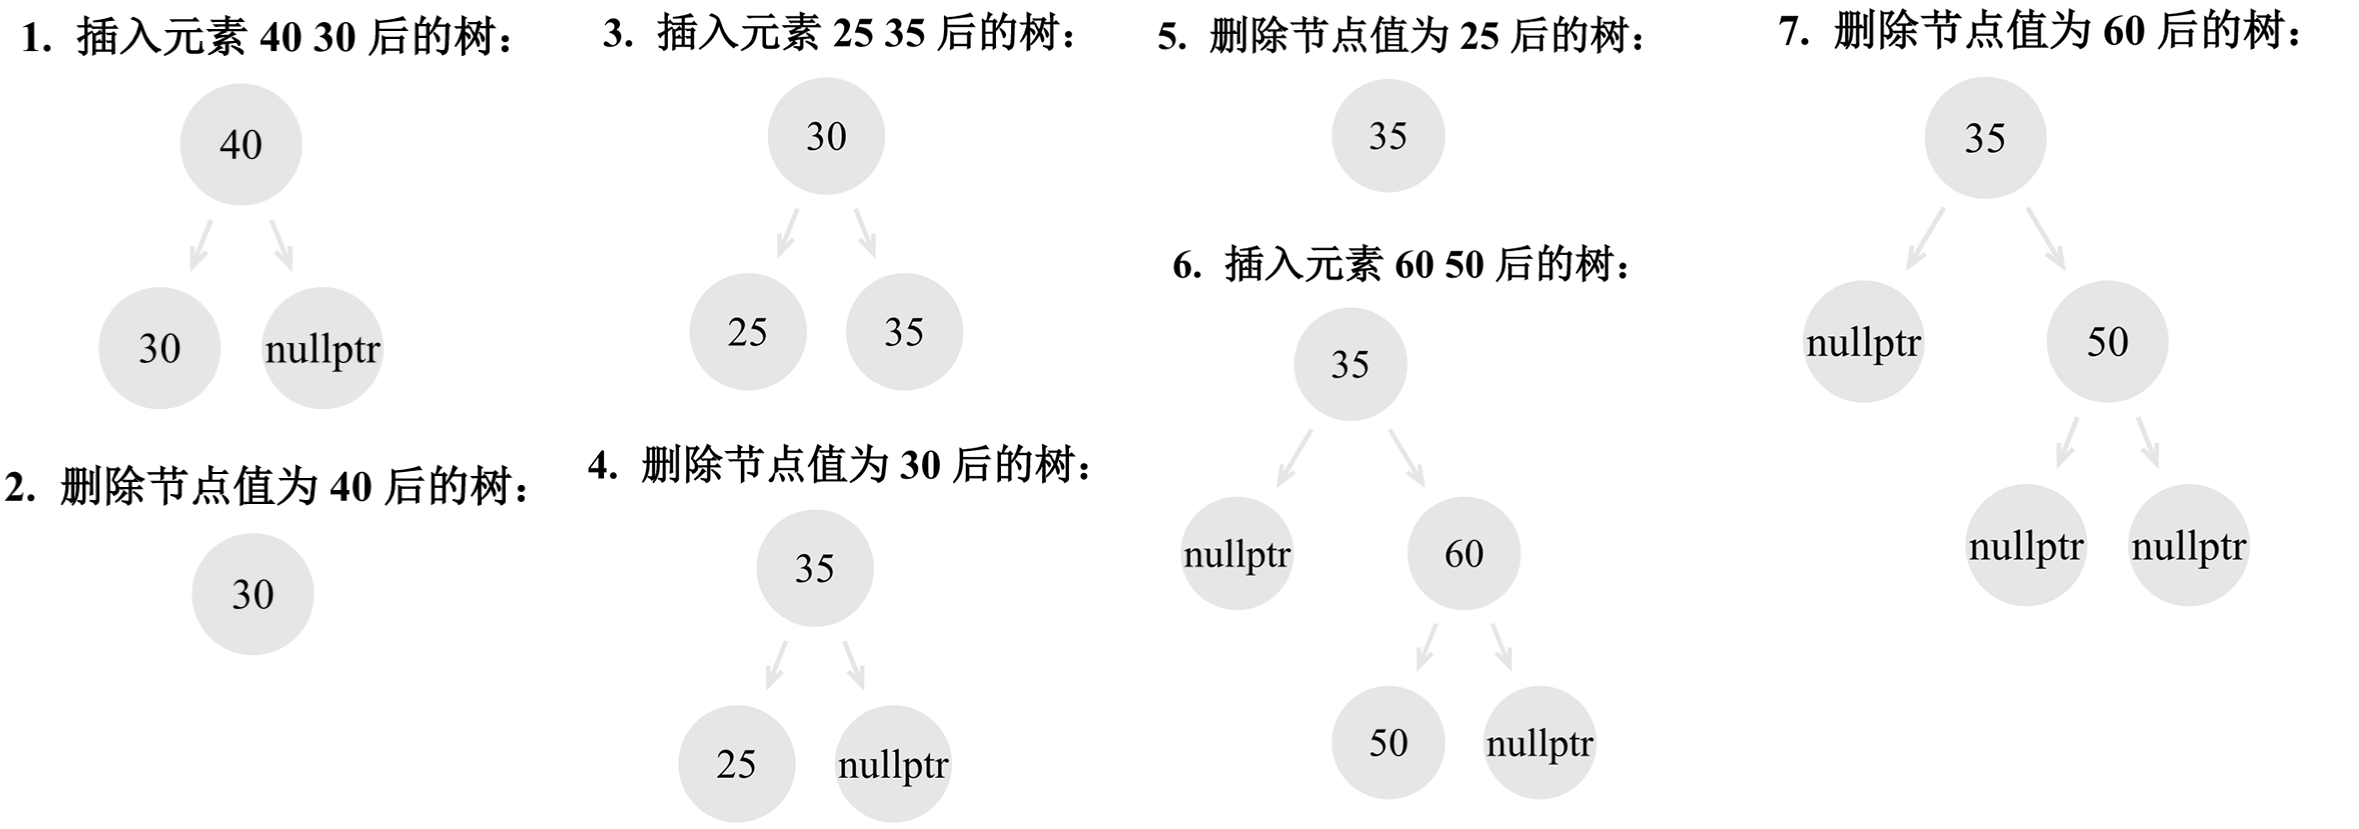
\includegraphics[width=0.9\linewidth]{./DS5_2.png}
    \caption{Module 2 程序对应的树的变化}
    \label{A4_prob}
\end{figure}

\begin{figure}[H]
    \centering
    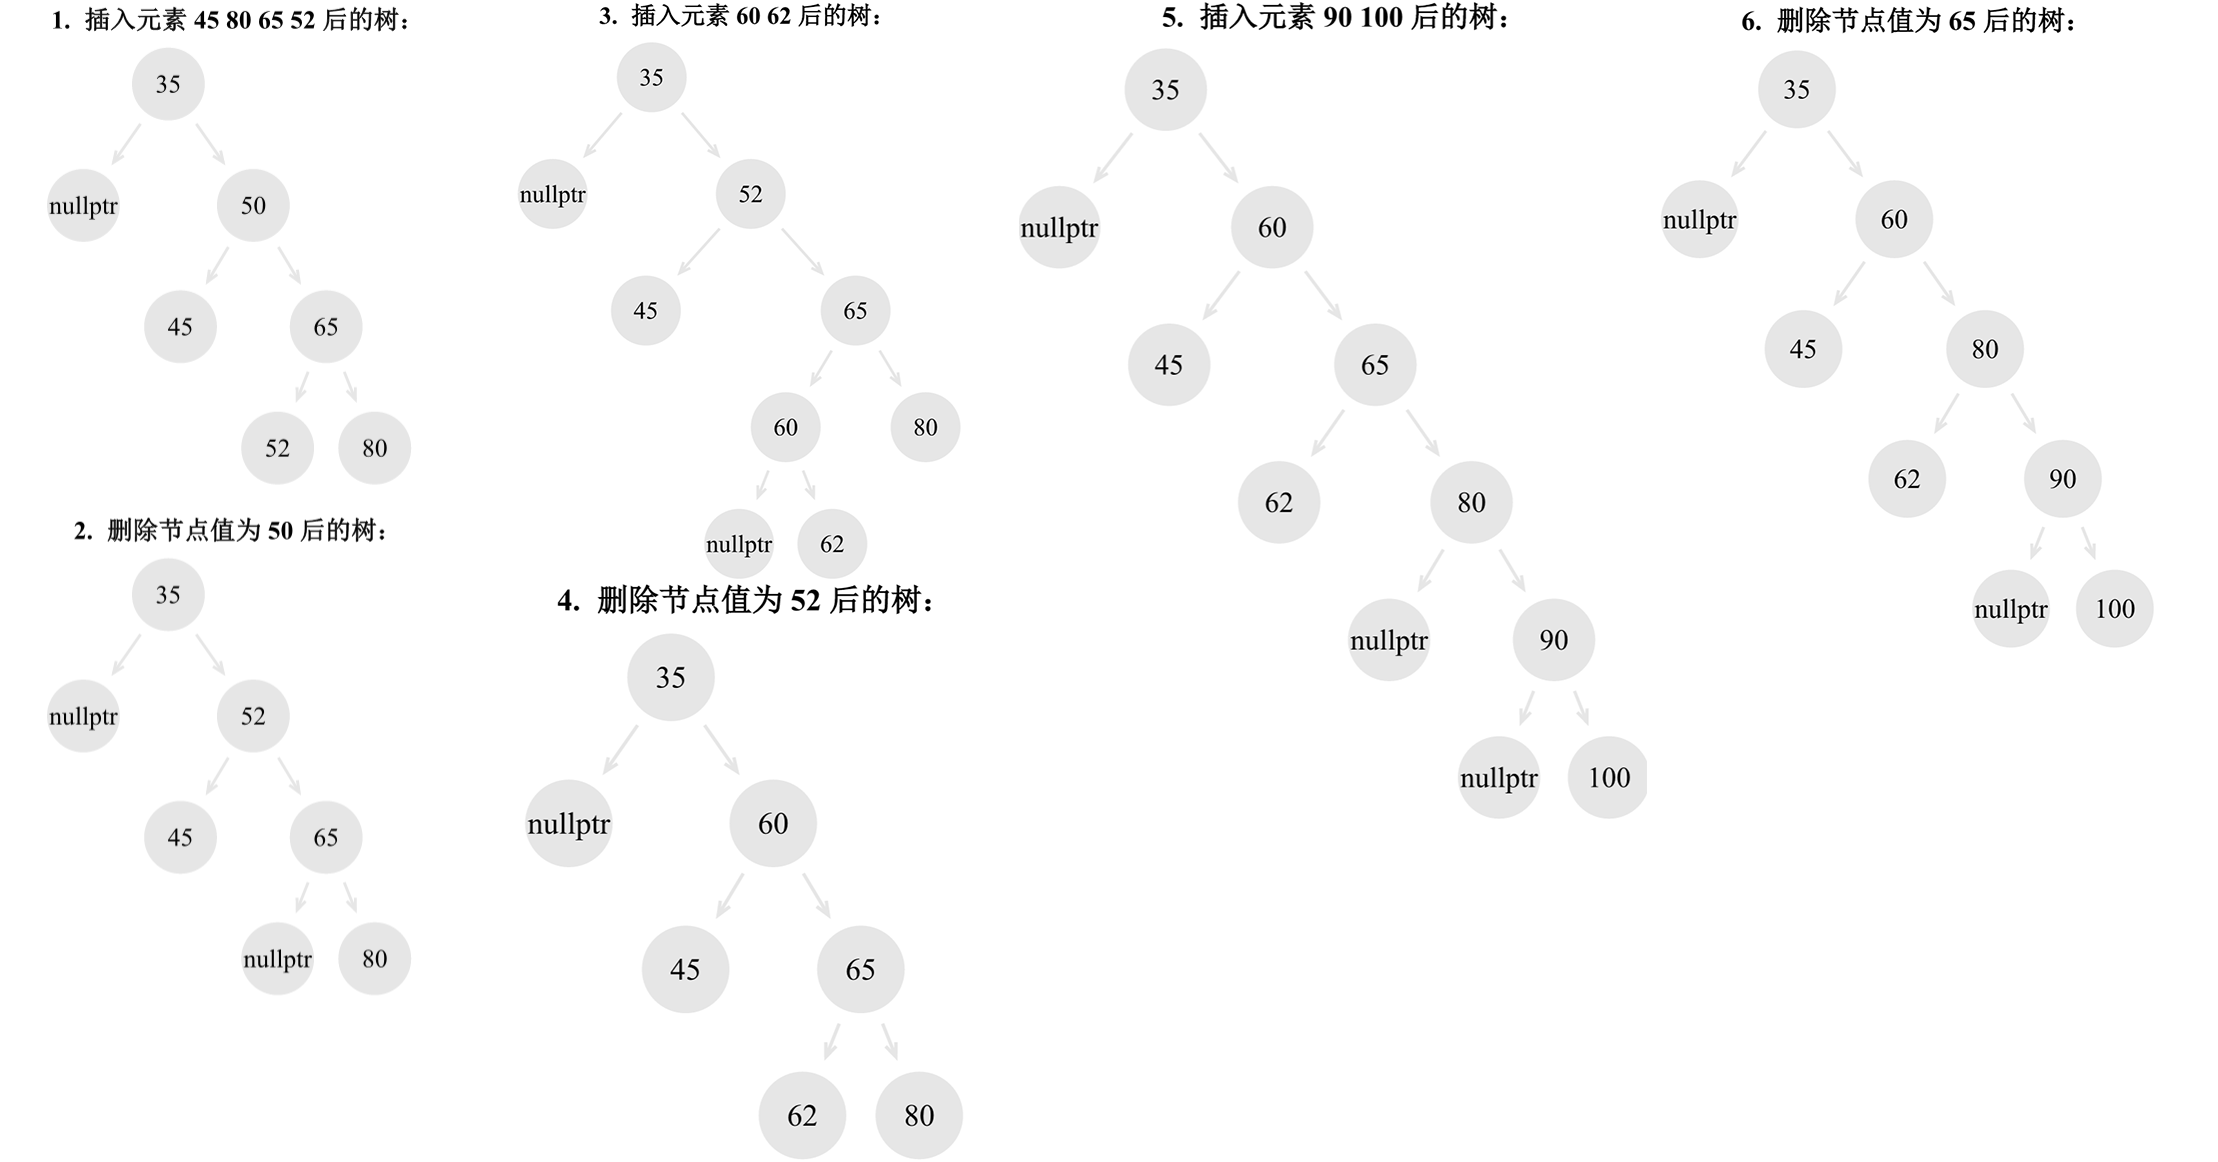
\includegraphics[width=1\linewidth]{./DS5_3.png}
    \caption{Module 3 程序对应的树的变化}
    \label{A4_prob}
\end{figure}


我用 \texttt{valgrind} 进行测试,发现没有发生内存泄露。
\begin{lstlisting}[ 
    language=c++,
    basicstyle=\ttfamily,
    breaklines=true,
    keywordstyle=\bfseries\color{Blue}, 
    morekeywords={}, 
    commentstyle=\itshape\color{black!50!white},
    stringstyle=\bfseries\color{PineGreen!90!black} 
    ]
    ==171299== 
    ==171299== HEAP SUMMARY:
    ==171299==     in use at exit: 0 bytes in 0 blocks
    ==171299==   total heap usage: 23 allocs, 23 frees, 74,144 bytes allocated
    ==171299== 
    ==171299== All heap blocks were freed -- no leaks are possible
    ==171299== 
    ==171299== For lists of detected and suppressed errors, rerun with: -s
    ==171299== ERROR SUMMARY: 0 errors from 0 contexts (suppressed: 0 from 0)
\end{lstlisting}


\end{document}

%%% Local Variables: 
%%% mode: latex
%%% TeX-master: t
%%% End: 
